\subsection{Ethereum Virtual Machine dan Smart Contracts}
\label{subsec:evm-smart-contract}

Ethereum Virtual Machine (EVM) adalah sebuah mesin komputasi yang serupa dengan mesin virtual lainnya seperti Java Virtual Machine (JVM) atau .NET Common Language Runtime (CLR). EVM adalah mesin \textit{Turing-complete}, yang berarti bahwa EVM dapat menjalankan kode apapun yang diberikan kepadanya, dengan batasan waktu dan biaya, yang dihitung dengan \textit{gas}. EVM menjalankan kode yang ditulis dalam bahasa pemrograman Solidity, yang kemudian dikompilasi menjadi EVM Bytecode, yang kemudian dijalankan di dalam EVM. EVM memiliki beberapa komponen, seperti \textit{world state}, \textit{storage}, \textit{memory}, \textit{stack}, dan \textit{program counter} yang saling berinteraksi untuk mengeksekusi Smart Contract Bytecode seperti pada gambar \ref{image:evm-architecture} \parencite{wood2014ethereum}.

\textit{Gas} adalah unit yang digunakan untuk mengukur biaya komputasi dan penyimpanan yang digunakan untuk menjalankan aksi di dalam Blockchain Ethereum. \textit{Gas} adalah komponen penting dalam Ethereum dan menjalankan peran sebagai \textit{buffer} antara harga dari Ethereum dan \textit{reward} untuk \textit{miner} dan sebagai pertahanan untuk serangan \textit{denial-of-service attacks}.

\begin{figure}[ht]
	\centering
	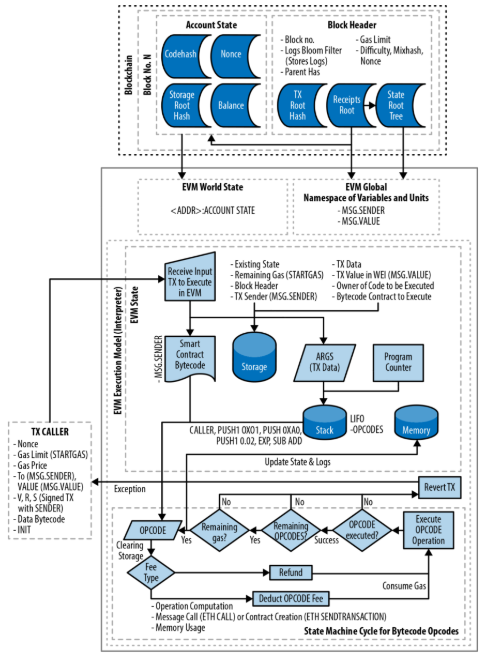
\includegraphics[width=0.7\textwidth]{resources/chapter-2/evm-architecture.png}
	\caption{Arsitektur EVM \parencite{antonopoulos2018mastering}}
	\label{image:evm-architecture}
\end{figure}

Smart Contracts adalah program yang ditulis untuk berjalan di atas Blockchain Ethereum. Smart Contracts adalah kode yang berjalan di dalam EVM, yang memungkinkan pengguna untuk membuat aturan dan logika yang akan dieksekusi secara otomatis ketika kondisi tertentu terpenuhi. Berikut adalah alur dari eksekusi Smart Contracts di dalam EVM:

\begin{enumerate}
	\item \textbf{Inisiasi Transaksi} \newline
	      Eksekusi dimulai saat ada transaksi yang memanggil fungsi pada Smart Contract yang mencakup data input, alamat Smart Contract, dan jumlah \textit{gas} yang dialokasikan.
	\item \textbf{Propagasi dan Validasi Transakksi} \newline
	      Transaksi akan dipropagasikan ke seluruh jaringan dan menunggu validasi awal untuk memastikan transaksi memenuhi kriteria.
	\item \textbf{Mempool dan Pemilihan oleh Validator} \newline
	      Transaksi yang telah diverifikasi akan dimasukkan ke dalam \textit{mempool}, yaitu \textit{queue} transaksi yang menunggu untuk dimasukkan ke dalam blok oleh validator (\textit{miner} dalam konsensus PoS).
	\item \textbf{Pembuatan dan Validasi Block} \newline
	      Transaksi yang terpilih akan disusun ke dalam sebuah blok yang kemudian divalidasi melalui mekanisme konsensus.
	\item \textbf{Eksekusi di EVM} \newline
	      Blok yang telah divalidasi akan ditambahkan ke dalam Blockchain, dan setiap transaksi di dalam blok tersebut akan dieksekusi oleh EVM. Proses eksekusinya dimulai dari kompilasi Smart Contract dalam Solidity menjadi Bytecode, lalu instruksi Bytecode akan dijalankan sesuai dengan biaya \textit{gas} yang dialokasikan, dan hasilnya akan disimpan secara permanan di dalam Blockchain.
	\item \textbf{Finalisasi dan Pencatatan di Blockchain} \newline
	      Hasil dari eksekusi Smart Contract akan dicatat di dalam Blockchain dan menjadi \textit{state} baru pada Blockchain.
\end{enumerate}

% Ethereum Virtual Machine (EVM) adalah sebuah lingkungan eksekusi untuk Smart Contracts di Ethereum, yang memungkinkan kode berjalan di seluruh jaringan Ethereum secara terdistribusi. EVM adalah sebuah mesin \textit{Turing-complete}, yang berarti bahwa EVM dapat menjalankan kode apapun yang diberikan kepadanya, dengan batasan waktu dan biaya yang ditentukan oleh \textit{gas} \parencite{wood2014ethereum}. EVM menjalankan kode yang ditulis dalam bahasa pemrograman Solidity, yang kemudian dikompilasi menjadi EVM Bytecode, yang kemudian dijalankan di dalam EVM. EVM memiliki beberapa karakteristik, seperti \textit{state}, \textit{storage}, \textit{memory}, \textit{stack}, dan \textit{program counter} \parencite{wood2014ethereum}.